\chapter{Introducción}
\label{ch:introduccion}

Para conocer la necesidad del proyecto, primero hay que introducir brevemente dos conceptos fundamentales dentro del proyecto, las aumentaciones web y dentro de ellas el editor WebMakeUp.

\section{Sobre las aumentaciones}
\label{sec:SobreAumentaciones}

Para describir de una buena manera en qué consiste una aumentación web o aumentación de navegador, primero se debe conocer su origen. El término aumentación web tiene como base el termino realidad aumentada (\emph{augmented reality}).

La realidad aumentada, tal y como se describe en Wikipedia \footnote{\url{http://en.wikipedia.org/wiki/Augmented_reality}} es la visión de la realidad a través de un dispositivo tecnológico donde se solapan elementos de la vida real con elementos virtuales. En la Figura \ref{fig:1-AugmentedReality} se muestra una aplicación de iOS donde mediante la cámara y el uso del GPS, consigue ubicar al usuario en el sitio donde se encuentra. En este caso la aplicación muestra la realidad, es decir, la calle; y además elementos virtuales, emplazamientos sobre algunos locales cercanos al lugar donde se encuentra, ofreciendo cierta información adicional.

\begin{figure}
\begin{center}
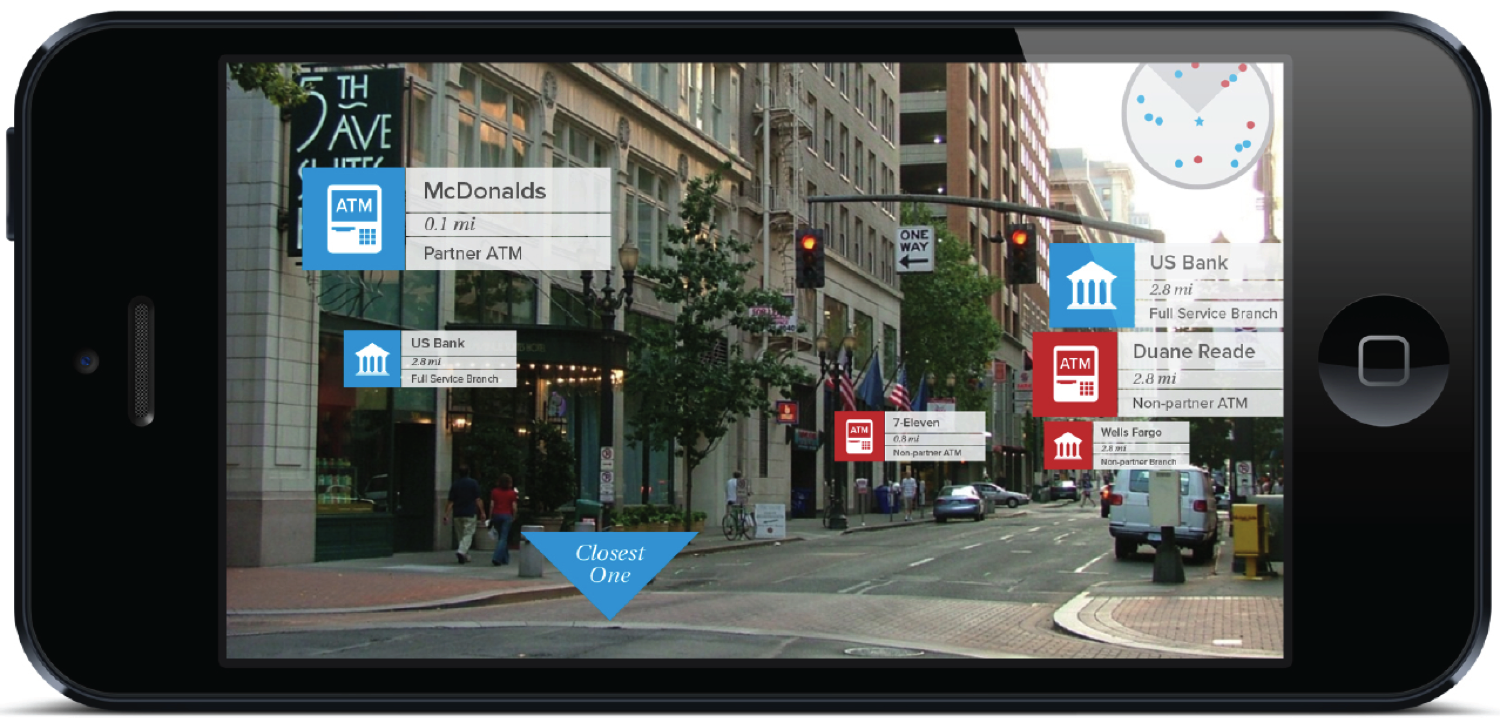
\includegraphics[width=0.85\textwidth]{figs/1-AugmentedReality.png}
\caption{Imagen sobre una aplicación de realidad aumentada.}
\label{fig:1-AugmentedReality}
\end{center}
\end{figure}

La aumentación web por tanto tiene un cometido muy similar al de la realidad aumentada, donde en este caso basándose en un sitio web concreto se realizan modificaciones virtuales, es decir, el sitio web real no se modifica, pero si se hace a la hora de presentarla al usuario con tal de satisfacer sus necesidades.

Estas necesidades pueden ser diferentes, pero habitualmente lo que se trata de mejorar es la focalización en las cosas que se quieren trabajar en el sitio web. Para ello se retiran elementos que no son necesarios y se cambian de sitio otros (dependiendo de la importancia que tengan para la labor que se esté desarrollando sobre ese sitio web).

En la arquitectura WWW (World Wide Web) existen dos agentes principales: el proveedor de contenidos (el servidor web) y el que renderiza (como por ejemplo el navegador web). El proveedor proporciona un contenido, habitualmente el mismo (o similar para todos los usuarios), que él considera adecuado para la mayoría de visitantes. Aun así las necesidades de todos los usuarios no son las mismas y puede que ese sitio web no permita realizar una navegación completamente satisfactoria en un usuario final.

Para resolver estas necesidades existen dos opciones. La primera es que lo haga el/los \emph{webmaster}. El webmaster será capaz de resolver las necesidades de cada uno de los usuarios ofreciendo contenido diferente acorde a esas necesidades, una labor costosa. La segunda solución es delegar parte de la responsabilidad al usuario.

Para ello se utilizan \emph{plugins}, extensiones, \emph{userscripts}, etc. Actualmente, la mayoría de navegadores admiten este tipo de tecnologías.


\section{Sobre WebMakeUp}
\label{sec:SobreWebMakeUp}

Las tecnologías que existen requieren de bastantes conocimientos de desarrollo software y conocimientos técnicos como pueden ser \emph{Javascript}, \emph{html} o \emph{css}. Habitualmente los usuarios carecen de ese tiempo, tanto para aprenderlos, como para desarrollarlos posteriormente.

De esta problemática surge la solución de realizar un editor DIY (\emph{Do-it yourself}), es decir, que un usuario sin necesidad de grandes conocimientos pueda realizar una aumentación. Con ella se pueden cubrir sus necesidades al acceder a un sitio web concreto. Mediante este editor bautizado como \textbf{WebMakeUp} se pueden crear \emph{mods} de un sitio web.

Un mod de un sitio web consiste en una modificación del contenido. Este contenido lo ofrece el proveedor del sitio web al que se accede. Los cambios que se pueden afectan al contenido Document Object Model (a partir de ahora DOM) HTML \footnote{¿Qué es el DOM HTML?: \url{http://www.w3schools.com/js/js_htmldom.asp}}, estilo o forma CSS, o interacción mediante Javascript. 

El contenido se relaciona con el concepto de Widget, es decir, un "trozo" de un sitio web, que puede abarcar desde toda la página, hasta un simple enlace, imagen, vídeo, etc. Un Widget puede tener o no interacción, y asociado a él va un estilo concreto. El usuario crea, modifica o destruye widgets para poder realizar una aumentación.

\begin{figure}
\begin{center}
\subfloat[TV Guía original]{
	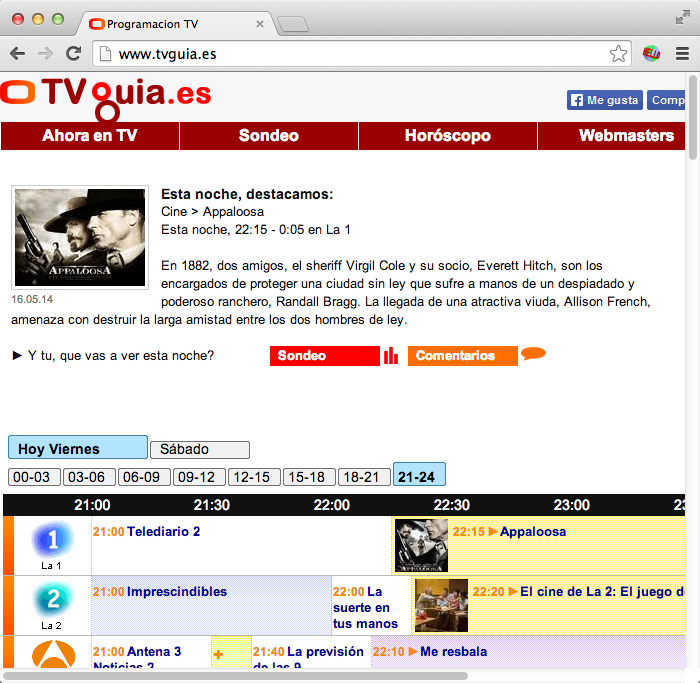
\includegraphics[width=0.5\textwidth]{figs/1-TVGuiaBefore.png}
	\label{fig:1-TVGuiaBefore}
}
\subfloat[TV Guia modificada]{
	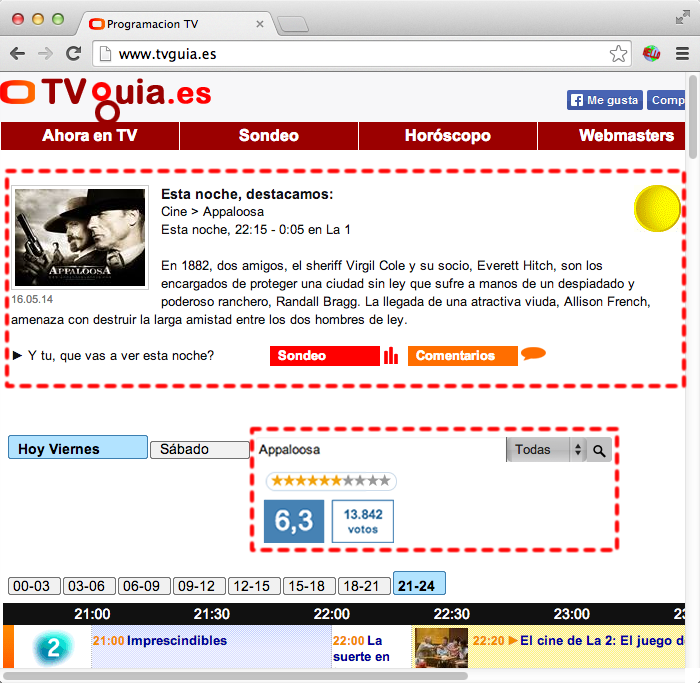
\includegraphics[width=0.5\textwidth]{figs/1-TVGuiaAfter.png}
	\label{fig:1-TVGuiaAfter}
}
\caption{\emph{www.tvguia.es} antes y después de ser modificada: se elimina el canal \emph{La 1} y se añaden ratings de filmaffinity sobre la película de la noche.}
\label{fig:1-TVGuia}
\end{center}
\end{figure}

Por ejemplo, en la Figura \ref{fig:1-TVGuia} se muestra la página web \url{www.tvguia.es} que ofrece la programación de las cadenas de televisión, donde se destaca en la parte superior la película de la noche. Mediante WebMakeUp se ha hecho un mod, donde se elimina la programación del canal \emph{La 1} y se añade el \emph{rating} (o puntuación) que le dan en \emph{www.filmaffinity.com} a la película destacada.

Gracias a este mod, se puede evitar ver información que no interesa (como puede ser la programación de un canal en concreto). También añadir información de otros sitios webs que interese dependiendo del contenido que sale en la propia web (como puede ser en este caso puntuación de la película obtenida de Filmaffinity).

El editor WebMakeUp se encarga de facilitar al usuario esta tarea ofreciendo un Lenguaje Específico de Dominio (\emph{Domain Specific Language}, a partir de ahora DSL), que trata de describir mediante un lenguaje lo más natural posible para un usuario final la manera de concebir una aumentación web.

Para definir este DSL hay que basarse en varias premisas. Una de ellas es la de poder realizarla en poco tiempo, en un \emph{coffee-break} o tiempo de tomar el café, unos 30 minutos. Estos coffee-breaks están condicionados a interrupciones por parte de compañeros de trabajo. Asimismo, los usuarios finales suelen ser bastante impacientes, quieren ver resultados rápido y sin necesidad de realizar grandes esfuerzos. También se ha tenido en cuenta el poco conocimiento del usuario, no conoce conceptos de programación, ni tiene la necesidad de ello, por tanto el editor tiene que ser lo más intuitivo posible y alejarse de la programación tratando de acercarse al lenguaje más afín al usuario.

Como buena muestra de estas propiedades, se ha desarrollado un pequeño vídeo\footnote{Vídeo de ejemplo de realización de una aumentación en WebMakeUp: \url{http://onekin.org/downloads/
public/WebMakeup/video.mov}} que describe cómo se realiza la aumentación web de la Figura \ref{fig:1-TVGuia}.

\section{Sobre el proyecto}
\label{sec:SobreProyecto}

Este documento refleja el trabajo realizado en tres áreas muy concretas de la aplicación WebMakeUp. Se han dividido en tres tareas, pero para garantizar la completa comprensión de las mismas y dado que tienen relación con el resto de la herramienta desarrollada, también se mencionarán otros aspectos a lo largo del propio documento.

El primero de los ámbitos en los que se trabaja está ubicado en las fases iniciales del proyecto. En ella hay que \textbf{buscar y analizar herramientas orientadas al usuario final} que tuvieran cabida con el concepto que se quería trabajar WYSIWYG (\emph{What You See Is What You Get}, es decir, que lo que ves es lo que vas a obtener). Para ello se tiene que investigar y analizar herramientas de desarrollo y editores orientados a usuarios finales (por ejemplo, Photoshop, muy relacionado con el concepto WYSIWYG). El objetivo, por tanto, es tratar de ajustarse a lo que se necesita, para poder describir el DSL y a su vez hacerlo \emph{user-friendly}, sencillo para el usuario.

Otra de las tareas importantes, que abarca gran parte del proyecto, \textbf{es la de describir las animaciones (o interacciones) de la aumentación} (conocido en WebMakeUp como modelo de orquestación u \emph{Orchestration}). Se opta en una primera versión por realizarlo de una manera gráfica mediante diagramas de transición de estados (\emph{State Transition Diagram}, a partir de ahora STD). Pero, finalmente, esta metodología no se ha decidido aplicar en base a estudios con usuarios finales, dada la complejidad que generaban. Para ello se decidió sustituir por la técnica basada en blinks (pestañeo), donde un Widget tiene dos estados \emph{enable} (mostrándose) o \emph{collapse} (ocultándose). La interacción con otros Widgets provocará esos blinks, alternando de un estado a otro.

El tercer aspecto, consiste en \textbf{transformar la aumentación en una extensión para el navegador Google Chrome}. Esto se hace a partir del modelo existente en el editor WebMakeUp. El usuario a medida que va trabajando con el editor, de manera interna se va generando un modelo de datos. El objetivo de esta tercera tarea es la de a partir de ese modelo generar una extensión funcional de Google Chrome. Con ello se evita tener que programar o conocer la plataforma. 

Cabe destacar que el proyecto tiene una dificultad clara en el desarrollo y la investigación, dada la temática, que es muy novedosa. Aun así, a lo largo del proyecto se trabajan otros valores añadidos, que se irán desglosando a lo largo del propio documento. Por ejemplo, metodologías ágiles de desarrollo, trabajos con herramientas colaborativas, etc.

\subsection{Estructura de la memoria}

La estructura de la memoria se divide en diferentes capítulos.

En el Capítulo \ref{cha:Antecedentes} se habla de los antecedentes del proyecto. Se comentan aspectos del marco de conocimiento que requiere este proyecto, las técnicas o herramientas que hay que conocer para el desarrollo del mismo, y la metodología de trabajo en grupo que existía.

El Capítulo \ref{cha:DOP} trata sobre los objetivos del proyecto. Se comentan las tareas y objetivos que se han definido para el cumplimiento del proyecto. A su vez, también se hace una breve mención de qué objetivos no se trataron y quedan como trabajo futuro.

El Capítulo \ref{cha:interacciones} habla sobre el desarrollo de la tarea introductoria de búsqueda de editores para ver cómo se podrían reflejar las aumentaciones de manera gráfica. Esto dará pie a la tarea de cómo reflejar las interacciones de aumentación, explicando las dos ideas que se han trabajado. La inicial, basada en diagramas de transición de estados, y la actual, basada en blinks.

El Capítulo \ref{cha:generador} se habla sobre el transformador de WebMakeUp. La idea de las interacciones con STDs, se utiliza para generar una extensión de Google Chrome a partir del modelo que proporciona WebMakeUp.

Además de lo que es el propio desarrollo del PFG, en el Capítulo \ref{cha:gestion} se comentarán los aspectos relacionados con la gestión del mismo, donde tienen cabida distintos aspectos de gestión, planificación, seguimiento y control, gestión de riesgos, de calidad, etc. Se observará cómo de satisfactoria ha sido la planificación y en qué medida se han cumplido los objetivos.

Se extraerán conclusiones en el Capítulo \ref{cha:conclusiones}, comentando cuáles han sido los objetivos, las enseñanzas y el trabajo futuro o las limitaciones del PFG.

Por último, comentar que existen diferentes anexos que complementan la lectura y completa la compresión del PFG. El Anexo \ref{sec:ActasDeReunion} presenta un acta de reunión de las múltiples que hay a lo largo del PFG. El Anexo \ref{sec:HerramientasGestion} se mencionan las diferentes herramientas de gestión que se han utilizado. El Anexo \ref{sec:ManualWebMakeUp} ofrece un breve manual de uso de WebMakeUp. Finalmente, el Anexo \ref{sec:CJS} describe ConstraintJS, una librería para implementar restricciones y máquinas finitas de estado (FSM) en Javascript.